\documentclass[11pt,a4paper]{article}
\newcommand{\docTitle}{Explorer Guide}
% preamble.tex --- shared LaTeX preamble for Choupo manuals
% Style: sober monochrome with subtle dark-blue accent for
% hyperlinks only.  Pedagogical boxes via tcolorbox.

% ---- Encoding, fonts, language --------------------------------------
\usepackage[utf8]{inputenc}
\usepackage[T1]{fontenc}
\usepackage{lmodern}
\usepackage[english]{babel}
\usepackage{microtype}
\usepackage{textcomp}

% ---- Layout ---------------------------------------------------------
\usepackage[a4paper, margin=2.4cm, headheight=15pt]{geometry}
\usepackage{fancyhdr}
\usepackage{titlesec}
\usepackage{enumitem}
\usepackage{longtable}
\usepackage{booktabs}
\usepackage{array}
\usepackage{tabularx}
\usepackage{multicol}
\usepackage{parskip}
\usepackage{needspace}
\usepackage{graphicx}

% ---- Code listings --------------------------------------------------
\usepackage{listings}
\usepackage{xcolor}

% Sober palette --- almost monochrome, one accent reserved for links
\definecolor{rulegray}{HTML}{888888}
\definecolor{lightgray}{HTML}{f4f4f4}
\definecolor{mediumgray}{HTML}{cccccc}
\definecolor{darkgray}{HTML}{555555}
\definecolor{accent}{HTML}{1c3a5a}

\lstdefinelanguage{dict}{
  morecomment=[l]{//},
  morecomment=[s]{/*}{*/},
  morestring=[b]",
}

\lstdefinelanguage{shell}{
  morecomment=[l]{\#},
}

\lstset{
  basicstyle=\ttfamily\footnotesize,
  backgroundcolor=\color{lightgray},
  frame=single,
  framerule=0.4pt,
  rulecolor=\color{mediumgray},
  numbers=none,
  showstringspaces=false,
  breaklines=true,
  breakatwhitespace=true,
  postbreak=\mbox{\textcolor{darkgray}{$\hookrightarrow$}\space},
  columns=fullflexible,
  keepspaces=true,
  xleftmargin=0.7em,
  framexleftmargin=0.7em,
  framextopmargin=0.5em,
  framexbottommargin=0.5em,
  commentstyle=\color{darkgray}\itshape,
  stringstyle=\color{black},
  language=shell,
  % No {---}/{--} -> en-dash rules: they mangle ASCII box art (the header
  % banner) and directory trees (|--...) and CLI --flags in listings.
  % Hyphens must stay literal in monospace.  Accents below ARE needed
  % (the listing font renders them via the LaTeX accent commands).
  literate={ã}{{\~a}}1 {á}{{\'a}}1 {â}{{\^a}}1
           {é}{{\'e}}1 {ê}{{\^e}}1
           {í}{{\'i}}1
           {ó}{{\'o}}1 {ô}{{\^o}}1 {õ}{{\~o}}1
           {ú}{{\'u}}1
           {ç}{{\c c}}1
           {·}{{\textperiodcentered}}1
}

% ---- PGFPlots (theory-guide figures) -------------------------------
\usepackage{pgfplots}
\pgfplotsset{compat=1.18}
\usetikzlibrary{arrows.meta, calc}

% ---- Boxes (pedagogical signposts) ----------------------------------
\usepackage[most]{tcolorbox}
\tcbuselibrary{breakable,skins}

\newtcolorbox{keyidea}{
  breakable,
  colback=lightgray,
  colframe=black,
  boxrule=0.4pt,
  arc=1pt,
  left=10pt,right=10pt,top=6pt,bottom=6pt,
  before upper={\noindent\textbf{\sffamily Key idea.}\quad},
}

\newtcolorbox{pitfall}{
  breakable,
  colback=white,
  colframe=darkgray,
  boxrule=0.4pt,
  arc=1pt,
  left=10pt,right=10pt,top=6pt,bottom=6pt,
  before upper={\noindent\textbf{\sffamily Common pitfall.}\quad},
}

\newtcolorbox{tryit}{
  breakable,
  colback=lightgray,
  colframe=darkgray,
  boxrule=0.4pt,
  arc=1pt,
  left=10pt,right=10pt,top=6pt,bottom=6pt,
  before upper={\noindent\textbf{\sffamily Try it now.}\quad},
}

\newtcolorbox{whatyoulllearn}{
  breakable,
  colback=white,
  colframe=black,
  boxrule=0pt,
  leftrule=2pt,
  arc=0pt,
  outer arc=0pt,
  left=10pt,right=4pt,top=2pt,bottom=2pt,
  before upper={\noindent\textit{\sffamily\small What you'll learn.}\quad},
}

% Worked example --- the pedagogical workhorse of the theory manual.
\newcounter{theoryexample}[section]
\renewcommand{\thetheoryexample}{\thesection.\arabic{theoryexample}}
\newtcolorbox{example}[1][]{
  breakable,
  colback=lightgray,
  colframe=black,
  boxrule=0.4pt,
  arc=1pt,
  left=10pt,right=10pt,top=6pt,bottom=6pt,
  title={\textbf{\sffamily Worked example~\thetheoryexample.}\enspace #1},
  fonttitle=\sffamily,
  coltitle=black,
  attach title to upper,
  before title={\refstepcounter{theoryexample}},
}

% Intuition --- a one-paragraph sense-making aside, marked by a left rule.
\newtcolorbox{intuition}{
  breakable,
  colback=white,
  colframe=black,
  boxrule=0pt,
  leftrule=2pt,
  arc=0pt,
  outer arc=0pt,
  left=10pt,right=4pt,top=2pt,bottom=2pt,
  before upper={\noindent\textit{\sffamily\small Intuition.}\quad},
}

% Link-back to a tutorial --- visual cue that this maps to a runnable case.
\newtcolorbox{tutoriallink}{
  breakable,
  colback=white,
  colframe=darkgray,
  boxrule=0pt,
  leftrule=2pt,
  arc=0pt,
  outer arc=0pt,
  left=10pt,right=4pt,top=2pt,bottom=2pt,
  before upper={\noindent\textbf{\sffamily\small Runnable case.}\quad},
}

% ---- Headers/footers ------------------------------------------------
\pagestyle{fancy}
\fancyhf{}
\renewcommand{\sectionmark}[1]{\markboth{\thesection\quad #1}{}}
\fancyhead[L]{\small\sffamily\nouppercase{\leftmark}}
\fancyhead[R]{\small\sffamily\thepage}
\fancyfoot[C]{\small\sffamily Choupo-2607}
\renewcommand{\headrulewidth}{0.3pt}
\renewcommand{\footrulewidth}{0pt}

\let\choupoSection\section
\renewcommand{\section}{\clearpage\choupoSection}

% ---- Section titles -------------------------------------------------
\titleformat{\section}
  {\Large\bfseries\sffamily}{\thesection}{0.8em}{}[\vspace{-0.4em}\rule{\linewidth}{0.3pt}]
\titleformat{\subsection}
  {\large\bfseries\sffamily}{\thesubsection}{0.8em}{}
\titleformat{\subsubsection}
  {\normalsize\bfseries\sffamily}{\thesubsubsection}{0.8em}{}

\titlespacing*{\section}{0pt}{2.0ex plus 1ex minus.2ex}{1.0ex plus.2ex}
\titlespacing*{\subsection}{0pt}{1.6ex plus 1ex minus.2ex}{0.8ex plus.2ex}

% ---- Hyperref last --------------------------------------------------
\usepackage[colorlinks=true,
            linkcolor=accent,
            citecolor=accent,
            urlcolor=accent,
            bookmarksnumbered=true,
            destlabel=true,        % \label{ch:cstr} -> PDF named destination "ch:cstr"
            pdfborder={0 0 0}]{hyperref}

% ---- Shortcuts ------------------------------------------------------
\newcommand{\code}[1]{\texttt{#1}}
\newcommand{\file}[1]{\texttt{#1}}
\newcommand{\dict}[1]{\texttt{#1}}
\newcommand{\cpp}{C\texttt{++}}

% Manual authorship is selected by each guide before loading this preamble.
% Properties/Theory: Vitor, Pedro, Miguel. All other guides: Vitor alone.
\newcommand{\manualauthors}{%
  \ifdefined\propertyTheoryAuthors
    V\'{\i}tor Geraldes, Pedro Mendes, and Miguel Rodrigues%
  \else
    V\'{\i}tor Geraldes%
  \fi}

% OpenFOAM-style manual front matter: title page, then a copyright/licence
% notice page.  No source-code banner belongs on manual covers.
\newcommand{\manualfrontmatter}[2]{%
  \begin{titlepage}
  \thispagestyle{empty}
  \vspace*{2.0cm}
  \begin{center}
  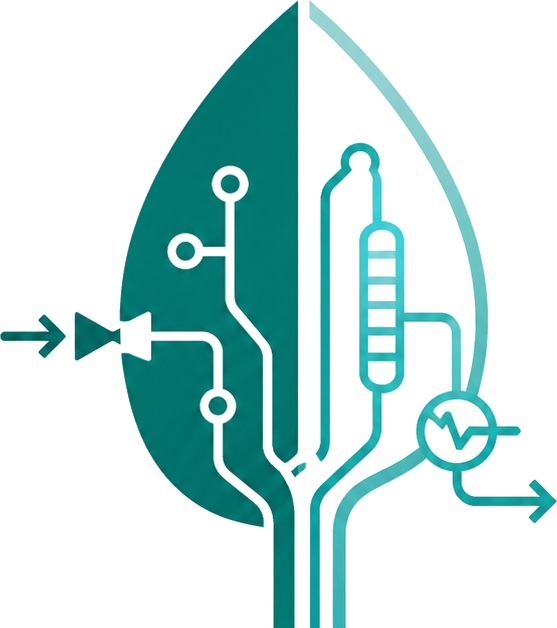
\includegraphics[height=4.0cm]{../gui/public/logo2-mark.png}\\[0.8cm]
  {\Huge\bfseries\sffamily Choupo}\\[0.35cm]
  {\Large\sffamily The Open Source Chemical Process Simulator}\\[1.3cm]
  {\Huge\bfseries\sffamily #1}\\[0.7cm]
  {Version 2607}\\[0.1cm]
  {30 June 2026}
  \end{center}
  \end{titlepage}

  \clearpage
  \thispagestyle{empty}
  \vspace*{1.2cm}
  \noindent Copyright \textcopyright{} 2026 \manualauthors.\\[0.3cm]
  \noindent Authors: \manualauthors.\\[0.3cm]
  \noindent This work is licensed under a Creative Commons
  Attribution-ShareAlike 4.0 International License.\\[0.3cm]
  \noindent Code examples, Choupo case files, and other machine-readable
  examples are licensed under GPL-3.0-or-later.\\[0.3cm]
  \noindent Typeset in \LaTeX.

  \vspace{1.0cm}
  \noindent\rule{\linewidth}{0.3pt}
  \noindent\footnotesize\textit{Acknowledgment.}\quad Choupo was conceived and
  architected by V\'{\i}tor Geraldes. Substantial parts of the initial
  implementation, documentation, and tutorial corpus were produced with
  assistance from Anthropic Claude Code using Claude Opus/Fable models. This
  guide is published under human curation, review, and editorial responsibility
  by \manualauthors.

  \clearpage
  \markboth{License}{License}
  \section*{License}
  \lstinputlisting[
    basicstyle=\ttfamily\tiny,
    frame=none,
    backgroundcolor=\color{white},
    breaklines=true,
    columns=fullflexible
  ]{cc-by-sa-4.0.txt}

  \clearpage
  \markboth{Trademarks}{Trademarks}
  \section*{Trademarks}
  #2
  \clearpage
}


\title{}
\author{}
\date{}

\begin{document}

\manualfrontmatter{Explorer Guide}{
Choupo is a trademark of TalentGround Lda.

Anthropic, Claude, and Claude Code are trademarks or registered trademarks of
Anthropic, PBC.
}

% =====================================================================
\section{What the Explorer is}

The Explorer is Choupo's \emph{interactive thermodynamics bench}: pick
components, pick a view, and SEE what the selected property models do ---
instantly, in the browser, with no case authoring at all.  It answers the
question that comes \emph{before} any simulation: \textbf{``what does this
thermodynamics look like?''}

It sits deliberately between two other surfaces:
\begin{itemize}[leftmargin=*,nosep]
  \item The \textbf{props bench} (\code{choupoProps} cases) asks the same
        questions \emph{reproducibly}: a case file, golden-locked numbers,
        validation blocks.  The Explorer is its sketchpad --- what you find
        here, you pin down there.
  \item The \textbf{simulators} consume the models the Explorer displays.
        A surprise in a flowsheet (an azeotrope, a scaling mineral, a
        runaway $\gamma$) is usually visible in the Explorer in thirty
        seconds.
\end{itemize}

Everything the Explorer draws is computed by the SAME C++ engine
(compiled to WebAssembly) with the SAME curated catalogue
(\file{data/standards/}) the solvers use.  There is no ``display model'':
if the Explorer shows an azeotrope at $x = 0.89$, the distillation column
will hit it at $x = 0.89$.

\section{The workflow}

\begin{enumerate}[leftmargin=*,nosep]
  \item \textbf{Pick components} in the left panel.  The list is the live
        catalogue; each card shows the data the component actually carries
        (criticals, $P^{\mathrm{sat}}$, $c_p$, formation --- and what it
        lacks).  Case-local components (from an open case's
        \file{constant/}) appear alongside, marked.
  \item \textbf{Pick a view}.  A lens that does not apply to the selection is
        \emph{removed} from the strip, not greyed out --- so what you see
        offered is what can be answered.  (The one reason-string you will meet
        belongs to the lens you are ALREADY on, when a change of components
        drifts the selection out from under it.)
  \item \textbf{Pick the method} where more than one applies ---
        activity model, equation of state, $P^{\mathrm{sat}}$ correlation.
        Overlaying two methods on the same axes is the fastest modelling
        lesson Choupo offers: the gap between the curves IS the modelling
        uncertainty.
  \item \textbf{Export}: every view is a Plotly figure (zoom, hover, save
        PNG) backed by numbers you can carry into a props case for the
        golden-locked version.
\end{enumerate}

\section{The views, one by one}

\subsection{The compound browser (the Explorer's landing)}
%  MOVED 2026-09-03: the catalogue IS the Explorer's landing now
%  (?workspace=explore); the property surfaces moved to
%  ?workspace=properties and keep a compound rail of their own.
%  Record: docs/design/one-tab-one-thing.md §8, amended in §8.7.
% Verified against gui/src/ui/explore/CompoundBrowser.tsx (hosted by
% gui/src/ui/ExploreWorkspace.tsx:2149) and gui/src/case/family.ts.
% Tree of folding groups: CompoundBrowser.tsx:86-95 (OPEN_BY_DEFAULT,
% FAMILY_THRESHOLD), groups derived from record facts: 63-82, display
% order: 84-85; families built and ranked: 337-344, family headers folded
% with their count: 355-358; search flattens the tree: 207; double click
% inspects: 244.  Classification rule: family.ts:37-50 (header), 105-132
% (familyOf: UNIFAC groups first, formula second, "(by formula)" suffix at
% 124, "No formula declared in the record" at 121).
The catalogue is a \emph{tree}, not a list.  Groups derived from each
record's own facts fold and unfold with their member count; the groups a
student charges to a vessel open by default, the combustion library, the
radicals and the synthetic test stand-ins start folded.  A group too large
for one screen is subdivided into \emph{families}, and the family comes from
the record, never from the name: first the \emph{declared UNIFAC groups}
(the highest-precedence group present decides --- an acid before an ester
before an alcohol, down to an alkane); only for a record with no group
decomposition, the \emph{elemental formula}, coarser and labelled so with a
``(by formula)'' suffix.  A record with neither is shown under \emph{``No
formula declared in the record''} --- a visible curation gap, never a guess.
Typing in the search box flattens the tree; a double click inspects a
component without changing the set.  The browser reads the catalogue; it
does not edit a record.

The browser is the left half of the Explorer's \emph{landing} --- the screen
\code{?workspace=explore} opens; its right half shows the record of whichever
compound you last touched --- identity, what the record carries, the curation
dossier's verdict --- and its \textbf{Explore properties} button opens the
property surfaces in a tab of their own, carrying the set in the address
(\code{?workspace=properties\&components=water,ethanol}), which makes an
exploration a link you can hand to somebody.  Neither tab needs the other: the
surfaces have their own door on the hub, keep a compound rail, and open
perfectly well with nothing selected,
and a component the address names but the catalogue cannot resolve is left
out of the set and said so, never dropped in silence.

\subsection{Property vs $T$/$P$ (scan)}
Any pure-component property --- $P^{\mathrm{sat}}$, liquid density,
$c_p$, viscosity, enthalpy --- swept over temperature or pressure, for one
or many components.  Use it to: check a correlation's range before trusting
it in a case; compare components; spot the nonsense that extrapolation
produces outside a fit's window (the guide's recurring lesson: a
correlation is DATA, and data has a domain).

\subsection{Pure phase diagram ($P$--$T$)}
The phase map of one substance: the vapour-pressure (saturation) curve from
low temperature to the critical point, and --- \emph{where the compound's data
reach that far} --- the sublimation and melting lines meeting it at the triple
point.  Expect water's negatively-sloped melting line (the anomaly), and the
supercritical region where the liquid/vapour distinction dissolves.
%  2026-09-21: the app's caption used to end "Solid region omitted" on EVERY
%  compound, including water, whose legend beside it carried "sublimation
%  (S-V)" and "fusion (S-L)".  It is now read off the CSV's own `curve` column
%  (gui/src/case/solidPhaseData.ts), so the sentence and the picture cannot
%  disagree.  Hence the conditional clause here: the solid region is drawn for
%  a compound that carries the data and honestly absent for one that does not,
%  and the caption says which.
The sublimation line needs the triple point and an enthalpy of sublimation;
the melting line needs, on top of those, an enthalpy of fusion and the volume
change on melting.  A compound whose record carries none of them gets the
liquid--vapour diagram alone, and the caption under the plot states which of
the three cases you are looking at, rather than leaving you to wonder whether
the solid was omitted or simply does not exist.

\subsection{Binary boiling envelope ($T$--$x$--$y$)}
The bubble and dew curves of a binary at fixed $P$.  This is where
azeotropes announce themselves: the curves touch, and no distillation can
cross the touching point.  Switch the activity model (ideal $\to$ NRTL
$\to$ UNIFAC) and watch the envelope bend --- ideal solutions cannot
azeotrope; real ones do.  If you ask for NRTL or Wilson on a pair the
catalogue has no parameters for, the engine \emph{refuses the run}
and names the pair: running that pair as ideal would answer a different
question from the one you asked.  UNIFAC needs no fitted pair and is the
usual way on.

%  A \subsection{Binary flash (x-y + lever rule)} stood here.  The binary
%  flash is a METHOD CONSTRUCTION -- an operating line and its intersection --
%  so by the criterion that moved McCabe-Thiele and the psychrometric chart on
%  2026-08-15 it belongs in EduTools, where the SAME construction had in fact
%  been built again on 2026-08-28 over the same gui/src/case/binaryFlash.ts
%  geometry.  The Explorer lens was removed on 2026-09-21; the EduTools tool
%  "Flash (operating line)" is the one home, and it carries the derivation.
%  This paragraph replaces it rather than deleting it silently, because the
%  same sentence ("the lever rule made visible") described a picture the lens
%  had already stopped drawing.
\subsection{Equilibrium curve $y(x)$}
The most familiar diagram in vapour--liquid equilibrium, and for a long time
the hardest to find here: the vapour in equilibrium with each liquid
composition, against the $y = x$ diagonal, at fixed $P$.  The distance from
the diagonal IS the separability --- where the curve touches it, no
equilibrium stage separates anything, which is what an azeotrope means
operationally.  It is the same engine run as the boiling envelope beside it,
read on different axes, so switching between the two costs nothing.
%  2026-09-21: this was NOT a lens.  It was the second option of a `View:`
%  SegmentedControl the plot component drew inside its own box -- a fourth
%  chrome home the lens strip never showed, with the SET pill overlaid across
%  its label -- and while it was showing, the strip still lit "T-x-y" and the
%  caption still described the boiling envelope.  Vitor reported the diagram
%  missing three times before anyone found the control.

Everything a student draws ON this curve --- a feed, an operating line, its
intersection, the lever arms --- is a graphical \emph{method}, and those live
in EduTools (\S\ref{sec:edutools} below), not here.  The Explorer draws the
property surface; EduTools draws the construction on it.

\subsection{$\gamma(x)$ --- activity coefficients}
The raw non-ideality of a binary: $\gamma_1, \gamma_2$ against composition,
with the infinite-dilution values $\gamma^\infty$ at the edges.
$\gamma > 1$: the pair dislikes mixing (positive deviation, minimum-boiling
azeotropes); $\gamma < 1$: association (maximum-boiling).  The
Gibbs--Duhem constraint ties the two curves together --- one cannot bend
without the other answering.  Read the pair note under the plot before you
read the curves: a parameter record may declare itself an \emph{assumption}
(\code{origin assumed}, null coefficients) rather than a fit to data, and then
the two flat lines at $\gamma = 1$ are Raoult's law wearing an NRTL label ---
the benzene--toluene pair in the standard catalogue is exactly that.

\subsection{Binary and ternary LLE}
Liquid--liquid splitting from the mixing Gibbs energy: $g_{\mathrm{mix}}(x)$
with the common-tangent construction (binary), and the ternary solubility
envelope with tie-lines (UNIFAC-predicted).  Expect the tangent points ---
not the minima --- to define the coexisting phases; that distinction is the
whole thermodynamics of demixing.

\subsection{Ternary boiling surface}
$T_{\mathrm{bubble}}$ over the composition triangle: valleys are
distillation boundaries, and azeotropes sit at the stationary points.

\subsection{Scaling (SI vs recovery)}
The membrane/brine screening view: concentrate a water composition over
recovery and watch each mineral's saturation index climb toward
$\mathrm{SI} = 0$ (the precipitation line).  The Davies-vs-Pitzer method
switch is the lesson: at high ionic strength the two activity models give
DIFFERENT scaling verdicts, and choosing one is an engineering decision.

\subsection{Equilibrium map (Gibbs)}
The chemical-reaction view: pick two or more gas-phase species (with plain
formulas --- the atom matrix is derived from them, glass-box) and a feed,
and get iso-lines of a product's equilibrium mole fraction over the
$T\times P$ plane.  The whole point is the tension it makes visible: for
ammonia ($\mathrm{N_2+3H_2\rightleftharpoons 2NH_3}$) the equilibrium
optimum sits cold and high-pressure, yet the labelled industrial window
sits hot --- where the catalyst can work.  Answers the beginner's real
confusion first (``where do I write the reaction?'' --- you don't; Gibbs
redistributes the ATOMS you fed, shown as a live element balance).
\emph{Click any cell} for its full equilibrium composition and the
ready-to-run \code{gibbsReactor} case dict --- the map is a case generator.
The \emph{advanced} toggle exposes the temperature-approach $\Delta T$
(the empirical closeness-to-equilibrium knob commercial tools hide); it snaps rather
than animates, and ghosts the $\Delta T = 0$ contours underneath so you
read the before/after, not a motion.  Unconverged cells are marked, never
interpolated.

\subsection{Steam tables (IF97)}
Saturation and superheat properties of water from IAPWS-IF97 ---
$h_f, h_g, h_{fg}$, entropies, volumes --- the backbone of every steam and
power-cycle case, browsable.

%  McCabe--Thiele and the psychrometric chart used to have their own
%  subsections here as Explorer views.  Both moved to EduTools on
%  2026-08-15 (gui/src/ui/ExploreWorkspace.tsx:20-24, 97-98: the Explore
%  workspace is PROPERTY-PURE, method constructions live in
%  MethodsWorkspace.tsx), and this guide went on describing them as
%  Explorer views for three weeks.  Retired 2026-09-03 by the coverage
%  sweep; they are reached from the EduTools workspace described next.
\subsection{EduTools (the Methods workspace)}\label{sec:edutools}
% Verified against gui/src/ui/MethodsWorkspace.tsx (criterion 36-41; zero
% physics in TS 42-48; chooser on a tool tab leads the chrome row, on a case
% tab it is a Select 96-101, 350, 518; TeachesLine 563; "Author -> copy
% propsDict" 618-635), gui/src/ui/methods/registry.ts (EDUTOOLS_LABEL 687;
% METHOD_TOOLS one home 125-137; planned entries visible, disabled
% 125-128), gui/src/ui/workspaces.ts (MODE_TABS 100-115: its own tab,
% independent of the flowsheet 56-62), gui/src/ui/WelcomeScreen.tsx:184-190
% (the hub opens it), docs/ai/gui-credo.md section 9 (line 410 on),
% docs/design/one-tab-one-thing.md.
Since 2026-08-15 the classical \emph{method constructions} live in their own
workspace, \textbf{EduTools}, split from the Explorer by one criterion:
\emph{a property surface answers ``what does this system's property look
like?''} (the Explorer); \emph{a method construction answers ``what does
the classical graphical method say about a design question?''} ---
the binary flash (operating line and lever rule), McCabe--Thiele, Kremser,
Rayleigh, $\varepsilon$-NTU, pinch composites, and derivation pages for the
property models.  Open it from the
hub's \textbf{EduTools} button: it is a tab of its own, needs no case, and
does not talk to the flowsheet.  A tool is chosen from the top row of the
tab; every tool carries a one-line ``teaches'' caption and its Theory Guide
link.  Every curve is an engine run (\code{choupoProps} in WebAssembly) over
a transient synthesized case --- \emph{zero physics in TypeScript}; the
staircase drawn on it is geometry.  Planned tools stay visible and
disabled, naming what will feed them.  It never writes a case: ``Author
$\to$ copy propsDict'' emits the dict for you to author on disk.

\subsection{Literature (``who measured this?'')}
% Verified against gui/src/ui/LiteratureWorkspace.tsx (header 1-27: the
% private ThermoML mirror installed by bin/choupo-thermoml sync, a reading
% list never a value; honest absence 21-27, 136-144; search rule: every
% word must match a compound, 160; the open case's components as chips,
% 168; hit = authors, year, title, journal, DOI link, measured properties,
% 199-230; closing line 240), gui/src/ui/workspaces.ts (Literature is a
% case-tab menu view, 135-137, offered for every case type and never
% without a case, 174-190), gui/src/ui/AppShell.tsx:418-419, 443-444.
Provenance is the differentiator, and this workspace puts its question one
click from the flowsheet.  With a case open, the tab's menu carries
\textbf{Literature}: type compound names (every word must match a compound
in the article) or click a chip for one of the case's own components, and
read who measured that system --- authors, year, title, journal, a DOI
link, and the properties measured.  It searches your \emph{private} mirror
of the NIST/TRC ThermoML Archive, installed once with
\code{bin/choupo-thermoml sync} on your own machine; the runtime never reads
it and the public site has no mirror, so there it shows the install
instructions instead.  That absence is a status, not an empty result:
\emph{``nobody measured this''} and \emph{``you have no mirror''} are
different sentences.  It is a \emph{reading list, never a value}: no number
is copied into a case or a record, and the only outbound action is opening
the article.  Read it and cite it --- never this index.

\section{Provenance and honesty rules}

The Explorer inherits the project's credo:
\begin{itemize}[leftmargin=*,nosep]
  \item \textbf{Every number has a source.}  Component cards show where each
        value came from; estimates carry their UNVALIDATED badge; nothing is
        silently filled in.
  \item \textbf{Irrelevant means absent.}  A view that cannot apply to the
        selection is removed from the strip rather than greyed --- never a dead
        button, and never a live one whose only possible answer is an error.
        Where a view you are already on stops applying, it says which
        requirement failed (component count, missing VLE data, missing UNIFAC
        groups).
  \item \textbf{The Explorer never writes.}  It reads the catalogue and the
        open case; promoting data, fitting parameters and locking goldens
        belong to the props bench and the curation tools.  Sketch here,
        commit there.
\end{itemize}

\section{From Explorer to case: the hand-off}

A typical session: you notice in the $T$--$x$--$y$ view that your solvent
pair azeotropes at 78\,\% --- so the simple column in your flowsheet cannot
deliver 99\,\% purity.  The hand-off is: (1) reproduce the envelope as a
props case (\code{propertyScanBinary}) so the finding is golden-locked;
(2) switch the flowsheet to the azeotrope-aware design (pressure-swing or
entrainer); (3) cite the Explorer finding in the case header.  The Explorer
is where you LEARN; cases are where knowledge is kept.

\end{document}
